\chapter{Basic Concepts}

\section{Performance Metrics} 

Para medir el performance de un modelo de \textit{Machine Learning} ya sea en problemas de clasificación o regresión, es posible utilizar distintas métricas de acuerdo a lo que nos importa medir en cada situación. 

\subsection{Classification Metrics}

\begin{figure}[H]
    \center
    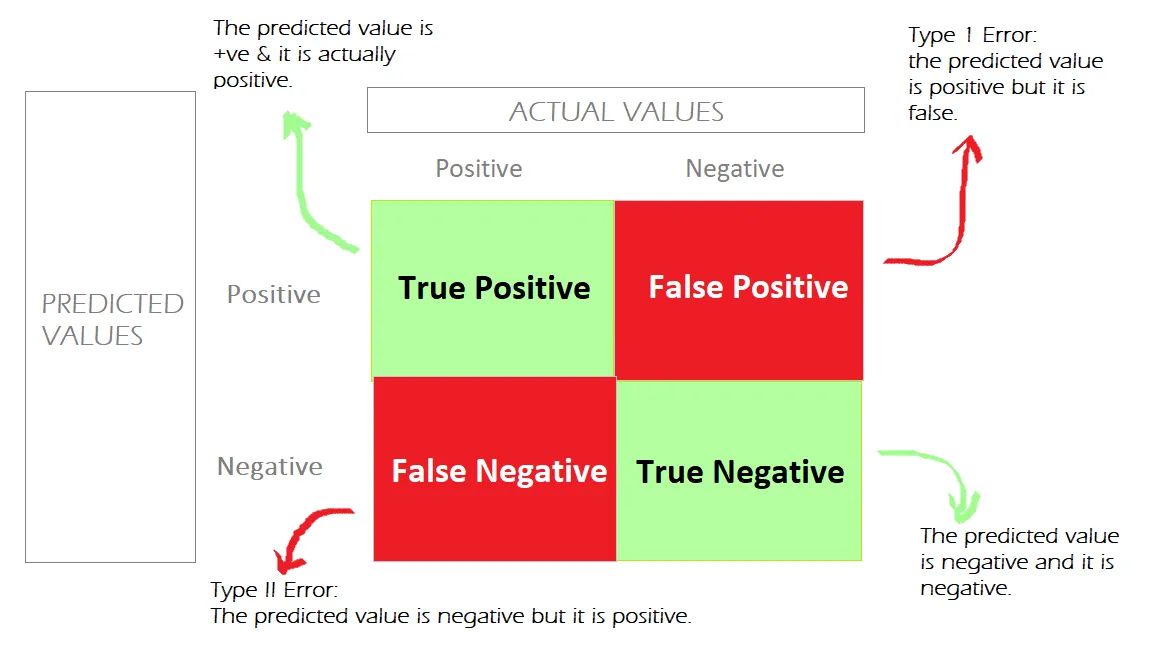
\includegraphics[scale=0.25]{notebooks/Basic/img/confusion_matrix_diagram.png}
    \caption{Confusion Matrix Diagram}
\end{figure}

En las métricas para problemas de clasificación, podemos encontrar
\begin{enumerate}
    \item \textbf{Accuracy:} Se define como el total de aciertos positivos y negativos sobre el total de predicciones. 
    $$ 
    \text{Accuracy} = \frac{TP + TN}{TP + TN + FP + FN}
    $$
    \item \textbf{Precision:} Este es el porcentaje de identificaciones positivas correctas en el total de identificaciones positivas. 
    $$
    \text{Precision} = \frac{TP}{TP + FP}
    $$
    \item \textbf{Recall: } Este es el porcentaje de identificaciones positivas correctas en el total de datos positivos. 
    $$ 
    \text{Recall} = \frac{TP}{TP + FN}
    $$
    \item \textbf{F1 - Score: } Esta métrica es la media armónica entre la precisión y el recall. 
    $$ 
    F_{1} = \frac{2}{\frac{1}{\text{precision}} + \frac{1}{\text{recall}}} = 2 \frac{\text{precision} \cdot \text{recall}}{\text{precision} + \text{recall}}
    $$
    Si alguna de las métricas tiene una mayor importancia dado el contexto del problema, podemos amplificarla por un valor $\beta$ de la siguiente forma
    $$ 
    F_{\beta} = (1 + \beta^2) \frac{\text{precision} \cdot \text{recall}}{\beta^2 \cdot \text{precision} + \text{recall}}
    $$
    Es decir, el recall es $\beta$ veces más importante que la precisión. 
\end{enumerate}

En problemas de clasificación binario, definir si un score se asigna al label positivo (1) o negativo (0) depende de un umbral (threshold) que se puede definir en base a qué métrica queremos optimizar. Lo anterior da origen a la curva \textit{Precision - Recall}

\begin{figure}[H]
    \center
    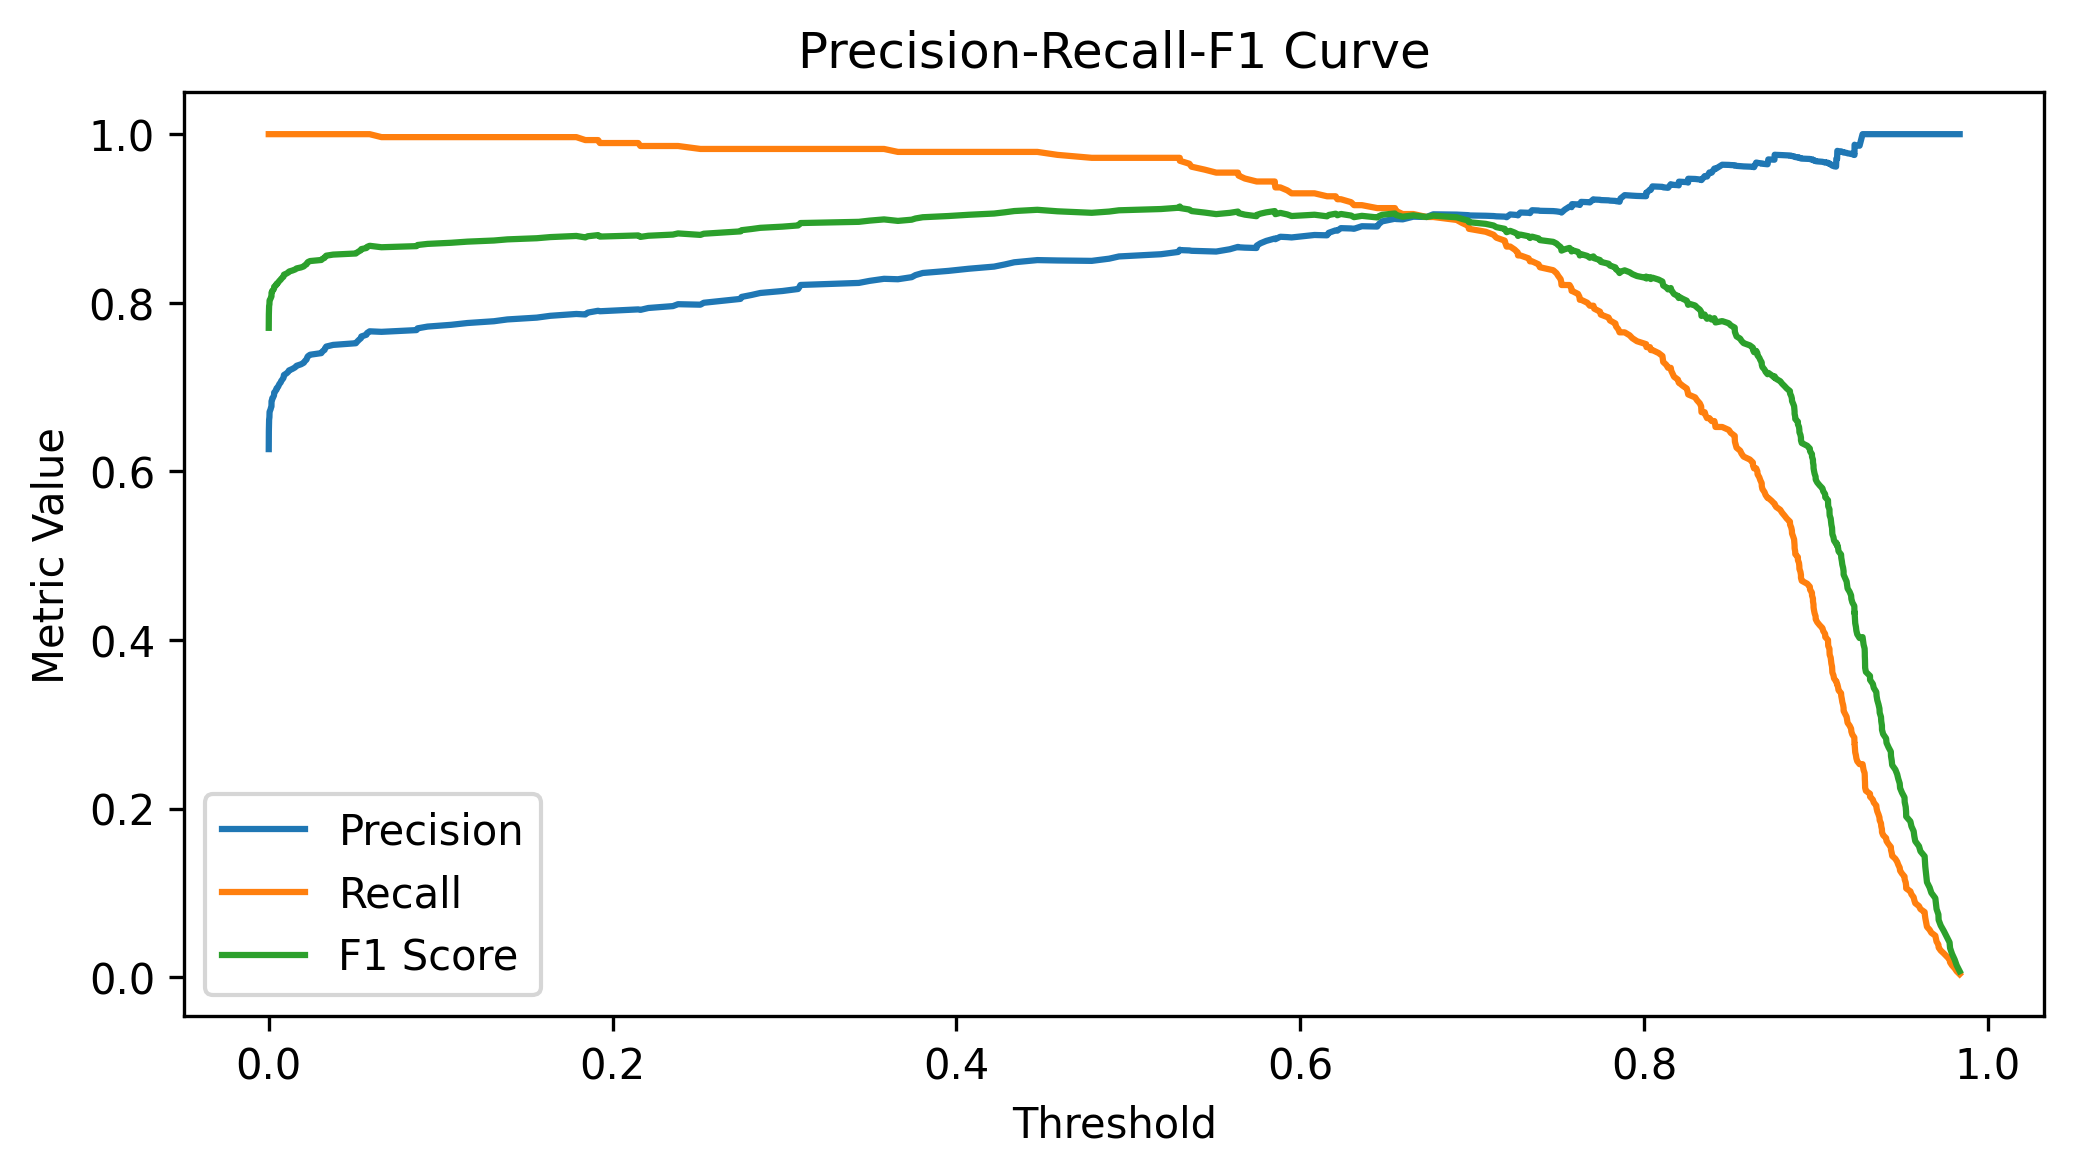
\includegraphics[scale=0.5]{notebooks/Basic/img/precision_recall_f1_curve.png}
    \caption{Precision-Recall-F1 Curve}
\end{figure}

Es fácil ver que el máximo de la métrica $F_{1}$ se alcanza en la intersección de la Precision y el Recall por la desigualdad AM-GM:
$$ 
\frac{n}{\frac{1}{x_1} + \dots + \frac{1}{x_n}} \leq \sqrt[n]{x_1 \dots x_n}
$$

Existen otras medidas que no dependen del threshold considerado, como: 

\begin{enumerate}
    \item \textbf{AUC: } Esta medida (\textit{Area Under the Curve)} se construye a partir de la tasa de TP y FP para todos los posibles umbrales de clasificación. 

    \begin{figure}[H]
    \center
    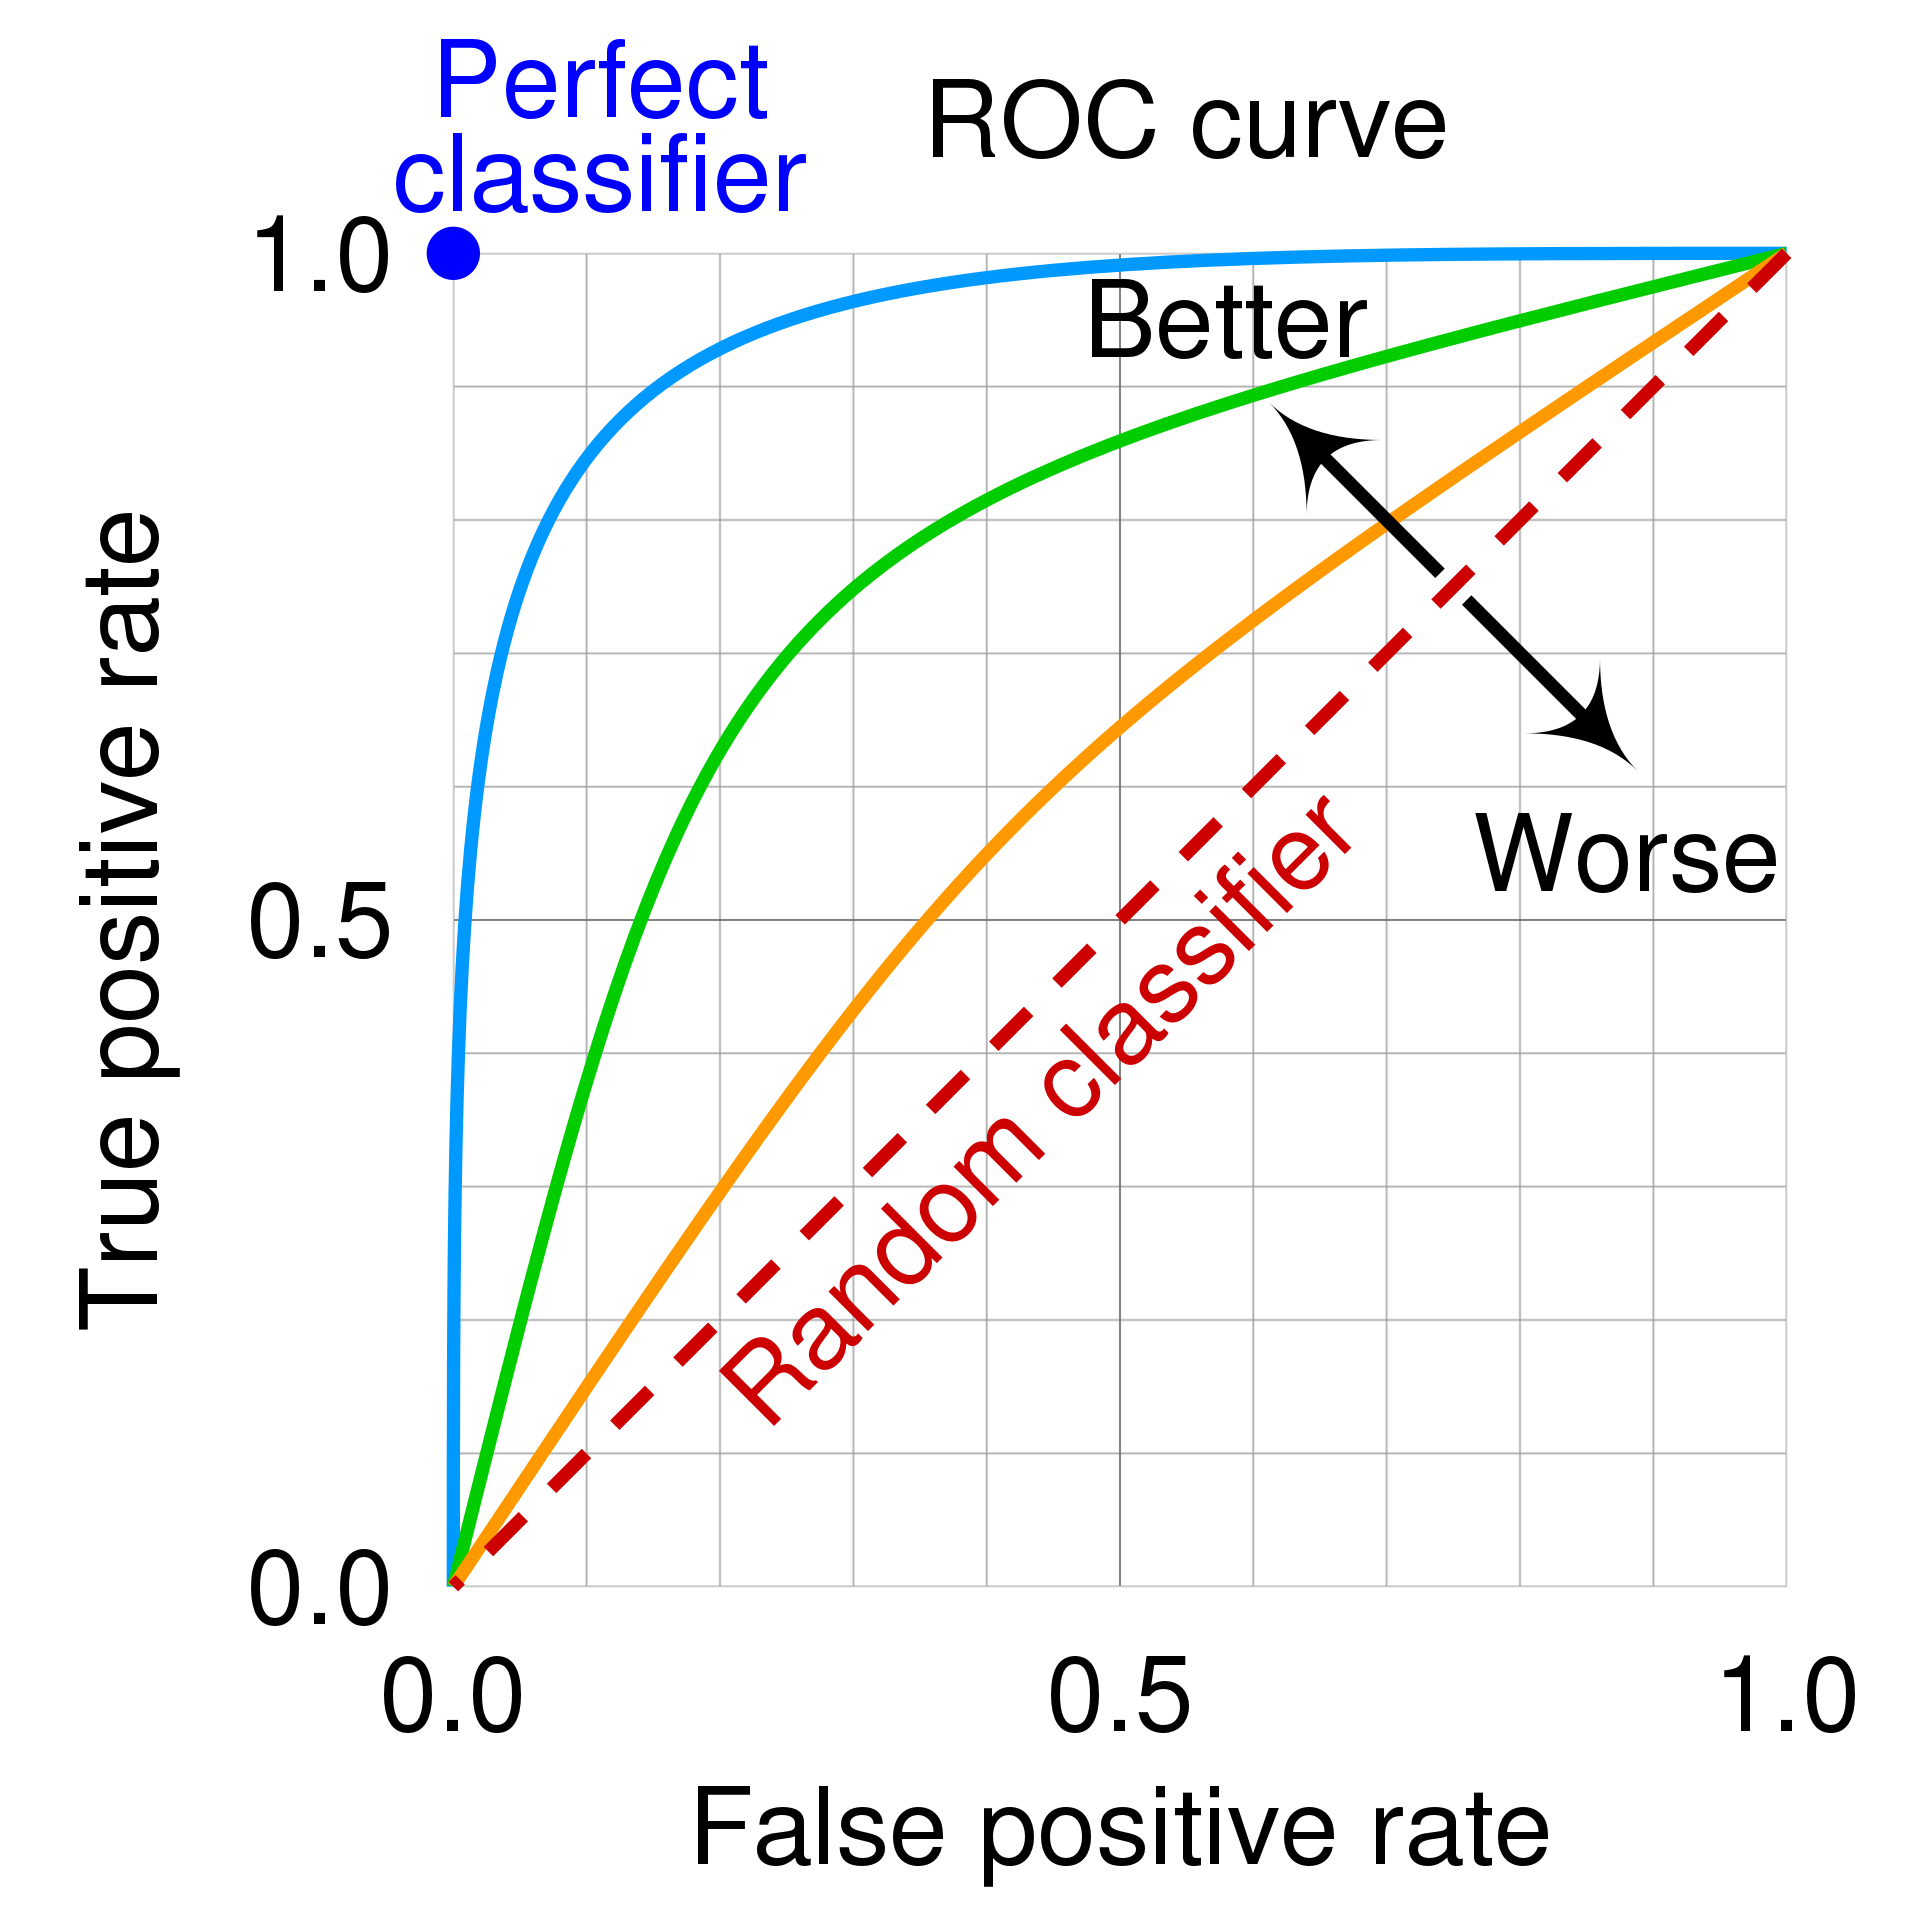
\includegraphics[scale=0.1]{notebooks/Basic/img/roc_curve_diagram.png}
    \caption{ROC Curve Diagram}
    \end{figure}

    El área por debajo de la curva ROC es lo que se conoce como AUC. Una mayor área indica un mejor rendimiento del modelo. 

    Una interpretación de esta medida, se puede entender cómo "La probabilidad de escoger el ejemplo con el label positivo dado que se presenta uno con label positivo y otro con label negativo", o bien, hablar del buen ordenamiento de los ejemplos positivos y los ejemplos negativos. 
    
    \item \textbf{Gini Index: } El índice de Gini se construye de manera similar al AUC, la conversión es directa según 
    $$ 
    \text{Gini} = 2 \cdot \text{AUC} - 1 
    $$
    \begin{figure}[H]
    \center
    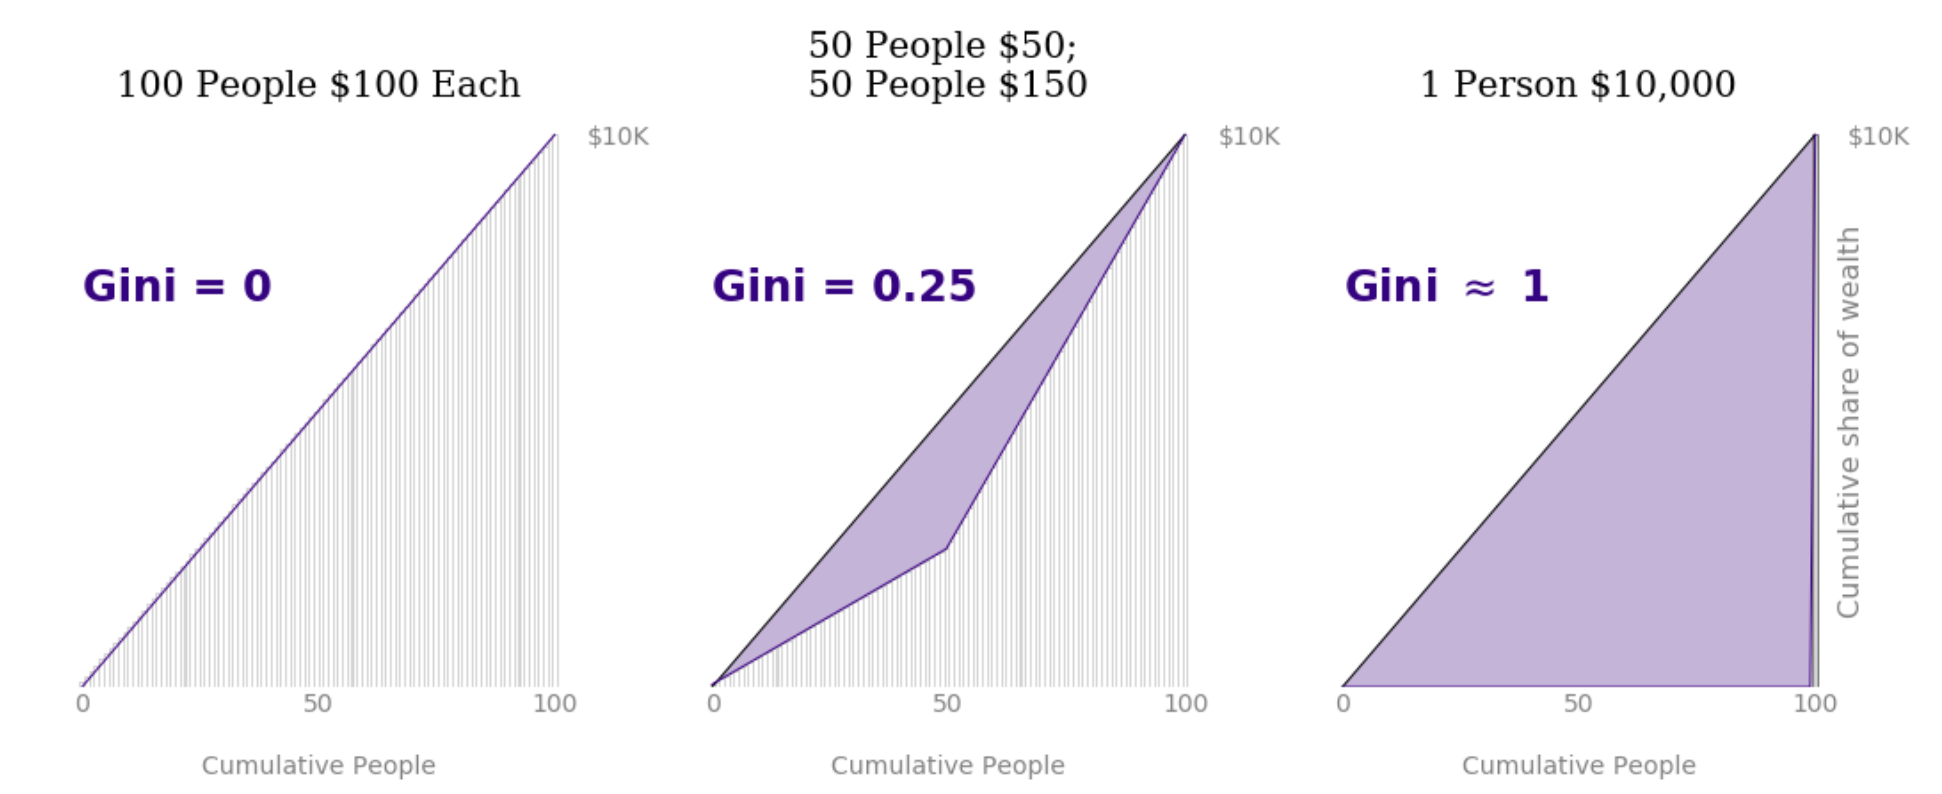
\includegraphics[scale=0.3]{notebooks/Basic/img/gini_diagram.png}
    \caption{Gini Diagram}
    \end{figure}
    
\end{enumerate}

\subsection{Regression/Forecasting Metrics}

Para problemas de regresión, es posible utilizar las siguientes métricas 
\begin{enumerate}
    \item \textbf{MSE}: El error cuadrático medio definido como 
    $$ 
    \text{MSE} = \sqrt{\frac{1}{N}\sum_{i=1}^N(y_i - \hat{y}_i)^2}
    $$
    \item \textbf{MAE}: El error absoluto medio definido como 
    $$ 
    \text{MAE} = \frac{1}{N}\sum_{i=1}^N|y_i - \hat{y}_i|
    $$
    \item \textbf{MAPE}: El error porcentual absoluto medio definido como 
    $$ 
    \text{MAPE} = \frac{1}{N}\sum_{i=1}^N \left | \frac{y_i - \hat{y}_i}{y_i} \right |
    $$
    \item \textbf{wMAPE}: El error porcentual absoluto medio pero ponderado según la magnitud de los datos. Esta métrica soluciona el problema de la gran variación porcentual que puede existir en datos de baja magnitud (Real: 1, Predict: 2 vs Real: 40, Predict: 50). 
    $$ 
    \text{wMAPE} = \frac{\sum_{i=1}^N w_i \cdot \left | \frac{y_i - \hat{y}_i}{y_i} \right |}{\sum_{i=1}^N w_i} = \frac{\sum_{i=1}^N |y_i| \cdot \left | \frac{y_i - \hat{y}_i}{y_i} \right |}{\sum_{i=1}^N |y_i|} =  \frac{\sum_{i=1}^N  \left | y_i - \hat{y}_i\right |}{\sum_{i=1}^N |y_i|}
    $$
    
    \item \textbf{R Squared}: El coeficiente de determinación $R^2$ es ampliamente utilizado para medir el poder predictivo de una regresión lineal. Es un valor que oscila entre 0 y 1 y está definido como 
    $$ 
    R^2 = 1 - \frac{SS_{\text{res}}}{SS_{\text{tot}}}
    $$
    Donde $SS_{\text{res}}$ es la suma de los cuadrados de las diferencias entre el valor real y la predicción. $SS_{\text{tot}}$ es la suma de los cuadrados de las diferencias entre el valor real y el valor medio de la variable (similar al cálculo de varianza). 

    \begin{figure}[H]
    \center
    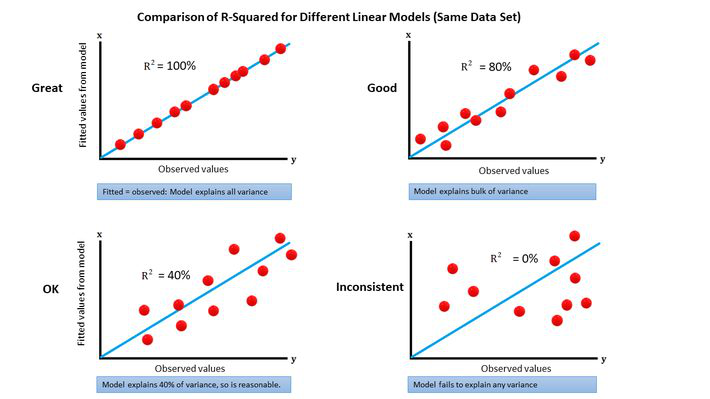
\includegraphics[scale=0.1]{notebooks/Basic/img/r_squared_diagram.png}
    \caption{R Squared Diagram}
    \end{figure}

    Existe una variación \textbf{Adjusted R Squared} que toma en consideración además la cantidad $M$ de features en el modelo. 

    $$
    R^2_{\text{Adjusted}} = 1 - \frac{(1-R^2)(N-1)}{N-M-1}
    $$

    La idea es controlar el overfitting al agregar más variables al modelo mejorando el $R^2$ pero no así el $R^2_{\text{Adjusted}}$.

    \item \textbf{Quantile Quality}: Esta métrica, especialmente útil para le medición de la calidad de un cuantil en forecast, se basa en la siguiente premisa: El $q_{0.9}$ debería en promedio, contener el 90\% de los datos. Se define de la siguiente manera: 

    $$
    QQ(q) = \frac{\sum_{i=1}^N (\mathds{1}_{y^{q}_i \geq y_i})}{N} - q
    $$
    Siendo $y^{q}_i$ la predicción de $y_i$ en el cuantil $q$. 
    
    
\end{enumerate}

\section{Bias vs Variance}

El dilema de \textit{Bias vs Variance} describe la relación entre la complejidad del modelo, la precisión de las predicciones y cómo éste se comporta al predecir datos nunca antes vistos. El error estimado de una predicción viene dado en términos generales por 
$$
\text{Expected Error} = (\text{Bias})^2 + \text{Variance} + \text{Irreductible Error}
$$
Así, un modelo que crece en complejidad reducirá su bias pero aumentará su varianza (extremo: overfitting) y a la vez, reducir la complejidad permitirá generalizar mejor reduciendo la varianza pero aumentando el bias (extremo: underfitting). 

\begin{figure}[H]
    \center
    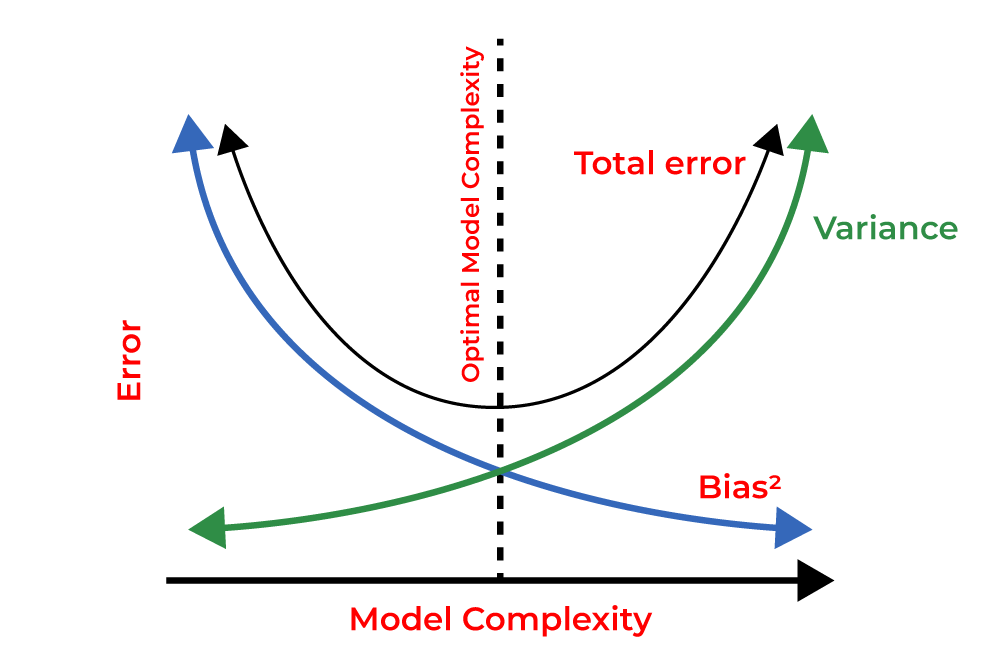
\includegraphics[scale=0.27]{notebooks/Basic/img/bias_vs_variance.png}
    \caption{Bias vs Variance Diagram}
\end{figure}
